\documentclass[11pt,a4paper]{article}
    \usepackage[margin=2.5cm]{geometry}
    \usepackage{enumitem}
    \usepackage{hyperref}
    \usepackage{tikz}
    \usetikzlibrary{arrows.meta,positioning,shapes.geometric}
    \title{Molecular Dynamics Tools}
    \author{CBBL Tools}
    \date{\today}

    \tikzset{
      methodbox/.style={
        rounded corners=6pt,
        draw=blue!50!black,
        line width=0.9pt,
        fill=blue!6,
        minimum width=13cm,
        text width=11.8cm,
        align=left,
        inner sep=8pt
      }
    }

    \begin{document}
    \maketitle

    \section*{Scope}
    This folder collects short teaching materials for molecular dynamics trajectory inspection and analysis. The current material is oriented to interactive notebooks based on MDAnalysis and NGLView, plus a minimal JSON parsing example.

    \section*{Material in this folder}
    \begin{itemize}[leftmargin=*]
\item \texttt{MDAnalysis\_traj\_ex1.ipynb}
\item \texttt{MDAnalysis\_traj\_ex2.ipynb}
\item \texttt{readJSON.py}
    \end{itemize}

    \section*{Method summary}
    \begin{itemize}[leftmargin=*]
\item \textbf{MDAnalysis trajectory inspection}. The notebooks load trajectories and topologies, expose atom selections, and inspect structural evolution frame by frame.
\item \textbf{Geometric measurements}. The atom-distance notebook illustrates how pairwise distances can be measured along a trajectory to summarize conformational changes.
\item \textbf{Interactive molecular visualization}. NGLView is used to render structures in the notebook and connect analysis code with visual interpretation.
\item \textbf{JSON parsing utility}. The Python helper reads a JSON export file and iterates over dictionary keys as a minimal data-ingestion example.
    \end{itemize}

    \section*{Method scheme}
    Figure~\ref{fig:summary} is drawn directly in LaTeX with TikZ. It is a compact conceptual map of the main workflows discussed in this folder.

    \begin{figure}[ht]
    \centering
    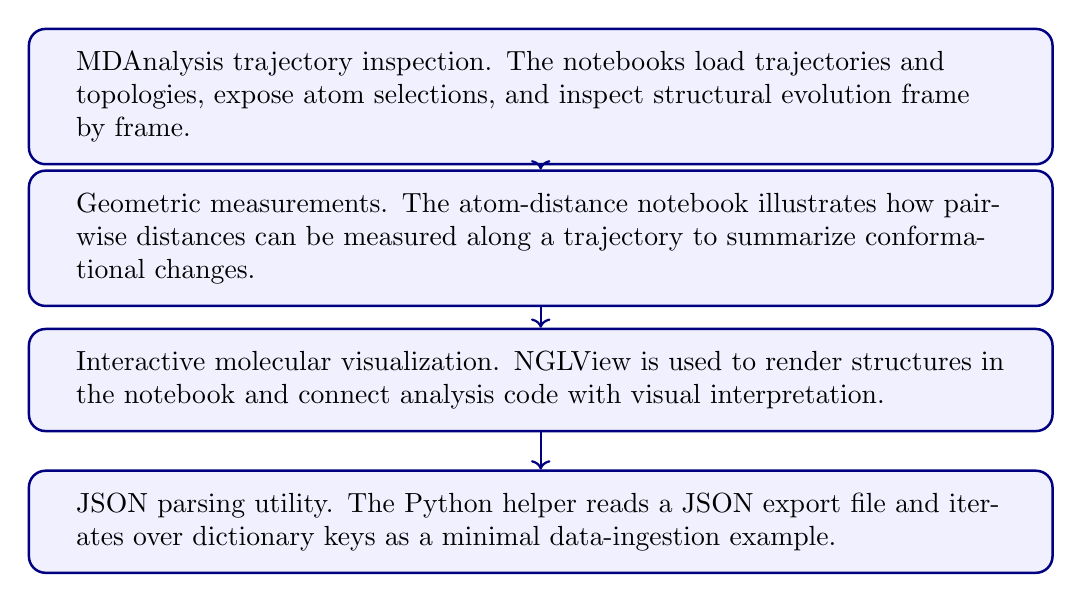
\begin{tikzpicture}[x=1cm,y=1cm]
    \node[methodbox] (m0) at (0,0.0) {MDAnalysis trajectory inspection. The notebooks load trajectories and topologies, expose atom selections, and inspect structural evolution frame by frame.};
    \node[methodbox] (m1) at (0,-1.8) {Geometric measurements. The atom-distance notebook illustrates how pairwise distances can be measured along a trajectory to summarize conformational changes.};
    \node[methodbox] (m2) at (0,-3.6) {Interactive molecular visualization. NGLView is used to render structures in the notebook and connect analysis code with visual interpretation.};
    \node[methodbox] (m3) at (0,-5.4) {JSON parsing utility. The Python helper reads a JSON export file and iterates over dictionary keys as a minimal data-ingestion example.};
    \draw[->, thick, color=blue!50!black] (m0.south) -- (m1.north);
    \draw[->, thick, color=blue!50!black] (m1.south) -- (m2.north);
    \draw[->, thick, color=blue!50!black] (m2.south) -- (m3.north);
    \end{tikzpicture}
    \caption{Conceptual scheme for the methods in the MDTools folder.}
    \label{fig:summary}
    \end{figure}

    \end{document}
